\documentclass[a4paper,11pt,pdftex]{article}

\usepackage[utf8]{inputenc}
%\usepackage[magyar]{babel} %needed in Hungarian reports
\usepackage{fancyhdr} %for the nice header
\usepackage{graphicx} %grapics input
\usepackage{tikz} %tikz figures

\usepackage{amsmath}
\usepackage{amsthm}
\usepackage{amssymb}

\newcommand{\R}{\mathbb{R}} 
\newcommand{\W}{W^{ss}_{loc}(0)}
\usepackage[a4paper,left=2.5cm,right=2.5cm,top=2.5cm,bottom=2.5cm,pdftex]{geometry} %margins

\usepackage{color}
\usepackage{url}
\usepackage{hyperref} %links
\hypersetup{
colorlinks=true,
linkcolor=blue,
urlcolor=blue,
citecolor=red
}

\rhead{NLDC II.}
\lhead{Homework 6}
\chead{B. Kaszas}

\setlength{\parskip}{0.5em}
\setlength{\parindent}{0em}

\title{Nonlinear Dynamics and Chaos II. \\ Homework 6}
\author{Kaszás Bálint}
\date{\today}

\begin{document}
\pagestyle{fancy}

\maketitle


\section*{Exercise 1}
Use the Lyapunov-Perron integral-equation approach discussed in class to prove the existence of a local
strong stable manifold $\W$ for two-dimensional, autonomous dynamical systems. In particular, consider a system of the form
$$
\dot{x} = f(x), \qquad x\in \mathbb{R}^2, \qquad f(0)= 0 \qquad \text{spect}[Df(0)] = \{ -\lambda_{ss}, -\lambda_s\},
$$

where $\lambda_s < \gamma < \lambda_{ss}$.

\emph{Solution}

Assume $\lambda_s > 0$, then $Df(0)$ is diagonalizable with the matrix $T$, formed from the eigenvectors of $Df(0)$, $T= [e_{ss}, e_{s}]$

$$
T^{-1}Df(0)T = \begin{bmatrix}
-\lambda_{ss} & 0 \\
0 & -\lambda_{s}
 \end{bmatrix}.
$$

Introducing a new variable $y$, defined by $x = Ty$, the differential equation reads,
\begin{equation}
\label{1}
\dot{y} = T^{-1}\dot{x} = \begin{bmatrix}
\dot{y}_{ss} \\ 
\dot{y}_{s}\end{bmatrix} = \begin{bmatrix}
-\lambda_{ss} y_{ss} + g_{ss}(y) \\
-\lambda_{s} y_{s} + g_{s}(y)
\end{bmatrix}    
\end{equation}
where $g_s$ and $g_{ss}$ are of order $O(|y|^2)$:
\begin{equation}
    \limsup_{|y|\to 0} \frac{|g_{s,ss}(y)|}{|y|^2}\leq K,
\end{equation}
for some $K$. 
To characterize the strong stable manifold $\W$, consider a modified form of (\ref{1}). Outside a small neighborhood $B_\delta:=[-\delta, \delta] \times [-\delta, \delta]\subset \R^2$, the vector field is smoothly changed to a linear one. 

This construction is done by using $C^\infty$ bump-functions $\psi_\delta : \R \to \R$, with the properties 

$$
\psi_\delta(r) = 1 \text{ for } |r|\leq \delta
$$
$$
\psi_\delta(r) \leq 1 \text{ for } \delta \leq |r|\leq 2\delta
$$
$$
\psi_\delta(r) = 0 \text{ for } 2\delta \leq |r|
$$
$$
|\psi_\delta(r)'| \leq \frac{K_0}{\delta}.
$$

Then, define the new functions, the components of the modified nonlinear part of the vector field (\ref{1}) as 

$$
G_{s, ss}: \R^2 \to \R
$$
$$
G_{s, ss}(y) := \psi_\delta(y_s)\psi_\delta(y_{ss})g_{s,ss}(y).
$$

The gradient of this function is (with the notation $\psi = \psi_\delta(y_{ss})\psi_\delta(y_s)$)
$$
\nabla G_{s, ss}(y) = g_{s,ss}(y)\begin{bmatrix}\psi_\delta(y_s)'\psi_\delta(y_{ss}) \\ \psi_\delta(y_{ss})'\psi_\delta(y_s) \end{bmatrix} + \psi(y) \nabla g_{s,ss}(y).
$$
The norm can be bounded by
$$
|\nabla G_{s, ss}(y) | \leq \sqrt{2}|g_{s,ss}|\frac{K_0}{\delta} + |\nabla g_{s,ss}(y)| \leq K_0 C \delta + C_1 \delta = K_2 \delta,
$$
because of the properties of the bump functions and we use the fact that $|g_{s,ss}|$ can be bounded by a quadratic function on the region $B_\delta$. 

The modified vector takes the form  
\begin{equation}
    \label{2}
    \begin{bmatrix}
    \dot{y}_{ss} \\
    \dot{y}_{s} 
    \end{bmatrix} = \begin{bmatrix} -\lambda_{ss} y_{ss} + G_{ss}(y)\\ -\lambda_{s} y_{s} + G_{s}(y)\end{bmatrix}.
\end{equation}
The strong stable manifold of system (\ref{2}) is $\overline{\W}$, which coincides with the strong stable manfifold of the original system on $B_\delta$. It is distinguished by the property, that trajectories on the manifold decay at least as fast as $e^{-\gamma t}$ for positive times:
$$
\W =\overline{\W}\cap B_\delta = \left\{ y_0\in B_\delta : \sup_{t\geq 0} e^{\gamma t}|F^t(y_0)| < \infty \right \}.
$$

To prove the existence of the strong stable manifold, we put system (\ref{2}) in a weak form, to make use of Banach's fixed point theorem. 

As seen in the lecture notes, the solutions of a system of the form
$$
\dot{x} = Ax + f(x,t)
$$

are the solutions to the integral equation
$$
x(t) = e^{A(t-t_0)}x_0 + \int_{t_0}^t e^{A(t-\tau)}f(x(\tau),\tau)d\tau.
$$

Applying this general form to system (\ref{2}), we have
\begin{align}
y_{ss}(t) &= e^{-\lambda_{ss}(t-t_{ss})}y_{ss}(t_{ss}) + \int_{t_0}^t e^{-\lambda_{ss}(t-\tau)}G_{ss}(y(\tau))d\tau \\
\label{5}
y_s(t) &= e^{-\lambda_s(t-t_s)}y_s(t_s) + \int_{t_0}^t e^{-\lambda_s(t-\tau)}G_s(y(\tau))d\tau. 
\end{align}

Assuming $\W$ is nonempty, pick an initial point $(y_{ss}(t_{ss}), y_s(t_s))\in \W$. It has the property 
$$
e^{\gamma \tau}|y_s(\tau)| \leq e^{\gamma \tau}|y(\tau)| < \infty, \text{ for } \tau \geq 0.
$$
Moreover, the norm of the first term in (\ref{5}) can be written as
$$
e^{-\lambda_s(t-t_s)}|y_s(t_s)| = |y_s(t_s)|e^{\gamma t_s} e^{-\lambda_s t}e^{-\lambda_s t_s}e^{-\gamma t_s} = |y_s(t_s)|e^{\gamma t_s} e^{-\lambda_s t} e^{(\lambda_s - \gamma)t_s}.
$$
Because $|y_s(t_s)|e^{\gamma t_s} e^{-\lambda_s t}$ stays bounded for given $t$, (using the previous line, with $\tau = t_s$) and $\lambda_s<\gamma$, we have 
$$
e^{-\lambda_s(t-t_s)}|y_s(t_s)| \to 0 \text{ as } t_s \to \infty.
$$

Then, we can choose the initial times to be $t_s = \infty$ and $t_{ss}=0$. Also, $y_{ss}(0)$ is the first coordinate of the initial point of the trajectory, when it enters $B_\delta$, that is, we can write $y_{ss}(0)=\delta$ to obtain the integral equations

\begin{align}
\label{6}
y_{ss}(t) &= e^{-\lambda_{ss}t}\delta + \int_{0}^t e^{-\lambda_{ss}(t-\tau)}G_{ss}(y(\tau))d\tau \\
\label{7}
y_s(t) &= - \int_{t}^\infty e^{-\lambda_s(t-\tau)}G_s(y(\tau))d\tau. 
\end{align}

Claim: The set 
$$
B : = \left \{ y(t): y\in C^0 ([0, \infty), B_\delta ), \quad  \sup_{t\geq 0} e^{\gamma t}|y(t)|\leq K <\infty \right \},
$$

equipped with the metric 
$$
d(y_1, y_2) := \sup_{t\geq 0} |y_1 - y_2|e^{\gamma t}. 
$$

becomes a complete metric space, on which the map
$$
\mathcal{F}_\delta  : B \to B,
$$
defined by the integral equations (\ref{6}), (\ref{7})
$$
\mathcal{F}_\delta (y) = \begin{bmatrix} e^{-\lambda_{ss}t}\delta + \int_{0}^t e^{-\lambda_{ss}(t-\tau)}G_{ss}(y(\tau))d\tau \\
- \int_{t}^\infty e^{-\lambda_s(t-\tau)}G_s(y(\tau))d\tau
\end{bmatrix}
$$
is a contraction mapping, that is, for $q<1$, 
$$
d(\mathcal{F}_\delta(y_1), \mathcal{F}_\delta(y_2))\leq q d(y_1, y_2). 
$$

First, we show that the map $d(y_1, y_2)$ is a metric, by showing that it satisfies the defining properties of a metric
\begin{align*}
    d(y_1, y_2) &= 0 \text{ if and only if } |y_1-y_2|=0 \Longleftrightarrow y_1=y_2 \\
    d(y_1, y_2) &= \sup_{t\geq 0} |y_1 - y_2|e^{\gamma t} = \sup_{t\geq 0} |y_2 - y_1|e^{\gamma t} = d(y_2, y_1) \\
    d(y_1, y_3) &= \sup_{t\geq 0} |y_1 - y_3|e^{\gamma t} \leq  \sup_{t\geq 0} (|y_1 - y_2| + |y_2 - y_3|)e^{\gamma t}= \\ &= \sup_{t\geq 0} |y_1 - y_2|e^{\gamma t} + \sup_{t\geq 0}  |y_2 - y_3|e^{\gamma t} = d(y_1,y_2) + d(y_2, y_3).
\end{align*}

In the usual metric, a sequence of uniformly continuous functions does have a continuous limit. If, in addition, the sequence of functions is also bounded in this weighted sense, the limit will also have this property, which means that B is complete. 

Next, we show that the map $\mathcal{F}_\delta$ defined above maps to 
$B$. 

\begin{align*}
|\mathcal{F}_\delta(y(t))| &\leq |y_s(t)| + |y_{ss}(t)| \leq |e^{-\lambda_{ss}t}\delta + \int_{0}^t e^{-\lambda_{ss}(t-\tau)}G_{ss}(y(\tau))d\tau| + |\int_{t}^\infty e^{-\lambda_s(t-\tau)}G_s(y(\tau))d\tau| \leq \\    
&\leq e^{-\lambda_{ss}t}\delta + \int_{0}^t e^{-\lambda_{ss}(t-\tau)}|G_{ss}(y(\tau))|d\tau + \int_{t}^\infty e^{-\lambda_s(t-\tau)}|G_s(y(\tau))|d\tau
\end{align*}
Using the mean value theorem, and the bound developed above, 
$$
|\nabla G_{s,ss}| \leq g_{s,ss} \leq K_2\delta, \qquad |G_{s,ss}(y_{s,ss})| \leq  K_2\delta |y_{s,ss}|
$$
\begin{align*}
|\mathcal{F}_\delta(y(t))| &= e^{-\lambda_{ss}t}\delta + \int_{0}^t e^{-\lambda_{ss}(t-\tau)}|G_{ss}(y(\tau))|d\tau + \int_{t}^\infty e^{-\lambda_s(t-\tau)}|G_s(y(\tau))|d\tau \leq \\
 &\leq e^{-\lambda_{ss}t}\delta + \int_{0}^t e^{-\lambda_{ss}(t-\tau)}K_2 \delta |y_{ss}(\tau)|d\tau + \int_{t}^\infty e^{-\lambda_s(t-\tau)}K_2 \delta |y_s(\tau )|d\tau 
\end{align*}
Multiply by $e^{\gamma t}$ and take the supremum
\begin{align*}
\sup_{t\geq 0}|\mathcal{F}_\delta(y(t))|e^{\gamma t} &\leq \sup_{t\geq 0} \left \{ \delta e^{(\gamma -\lambda_{ss}) t}  + \int_{0}^t e^{-\lambda_{ss}(t-\tau)}K_2 \delta |y_{ss}(\tau)|e^{\gamma t}d\tau + \int_{t}^\infty e^{-\lambda_s(t-\tau)}K_2 \delta |y_s(\tau )|e^{\gamma t}d\tau \right \} \leq  \\
& \leq \sup_{t\geq 0} \left \{ \delta + \int_{0}^t e^{-\lambda_{ss}(t-\tau)}K_2 \delta |y_{ss}(\tau)|e^{\gamma \tau} e^{-\gamma \tau }e^{\gamma t}d\tau + \int_{t}^\infty e^{-\lambda_s(t-\tau)}K_2 \delta |y_s(\tau )|e^{\gamma \tau} e^{-\gamma \tau }e^{\gamma t}d\tau\right \} \leq \\
&\leq \sup_{t\geq 0} \left \{ \delta +  K_2 \delta K\int_{0}^t e^{(t-\tau)(\gamma - \lambda_{ss})} d\tau +  K_2 \delta K\int_{t}^\infty e^{(t-\tau)(\gamma - \lambda_s)} d\tau\right \}
\end{align*}
After carrying out the integrals, and using $\gamma -\lambda_{ss} < 0$ and $\gamma-\lambda_s> 0$
\begin{align*}
\sup_{t\geq 0}|\mathcal{F}_\delta(y(t))|e^{\gamma t} &\leq 
\sup_{t\geq 0} \left \{ \delta +  K_2 \delta K \left [ \frac{1}{\lambda_{ss} - \gamma}e^{(t-\tau)(\gamma - \lambda_{ss})}\right]_0^t + K_2 \delta K \left [ \frac{1}{\lambda_{s} - \gamma}e^{(t-\tau)(\gamma - \lambda_{s})}\right]_t^\infty \right \}  = \\
&=  \sup_{t\geq 0} \left \{ \delta +  K_2 \delta K  \frac{1 - e^{t(\gamma - \lambda_{ss})}}{\lambda_{ss} - \gamma} + K_2 \delta K \frac{1}{\gamma - \lambda_{s} }\right \} \leq \\
& \leq \delta +  K_2 \delta K \left( \frac{1}{\lambda_{ss} - \gamma} + \frac{1}{\gamma - \lambda_{s} }\right) = K \left[\frac{\delta}{K}+K_2 \delta \left( \frac{1}{\lambda_{ss} - \gamma} + \frac{1}{\gamma - \lambda_{s} }\right) \right ]
\end{align*}
Choosing $\delta$, such that
$$
\delta \leq \frac{1}{\frac{1}{K}+K_2 \left( \frac{1}{\lambda_{ss} - \gamma} + \frac{1}{\gamma - \lambda_{s} }\right) }
$$
guarantees that 
$$\sup_{t\geq 0}|\mathcal{F}_\delta(y(t))|e^{\gamma t} \leq K < \infty,$$
which shows that the image of a function $y\in B$ under the functional $\mathcal{F}$ is still in $B$. 

So far we have established that $B$ is a complete metric space and $\mathcal{F}$ is a map from $B$ to $B$. To show that $\mathcal{F}$ is a contraction mapping, consider the difference between two  image-points in $B$

\begin{align*}
    |\mathcal{F}(y_1) - \mathcal{F}(y_2)| &= \left \vert\int_{0}^t e^{-\lambda_{ss}(t-\tau)}[G_{ss}(y_1(\tau)) - G_{ss}(y_2(\tau))]d\tau \right \vert +  \left \vert \int_{t}^\infty e^{-\lambda_s(t-\tau)}[G_{s}(y_1(\tau)) - G_{s}(y_2(\tau))]d\tau \right \vert \leq \\
    & \leq \int_{0}^t e^{-\lambda_{ss}(t-\tau)}|[G_{ss}(y_1(\tau)) - G_{ss}(y_2(\tau))]|d\tau  +  \int_{t}^\infty e^{-\lambda_s(t-\tau)}|[G_{s}(y_1(\tau)) - G_{s}(y_2(\tau))] | d\tau \leq \\
    & \leq \int_{0}^t e^{-\lambda_{ss}(t-\tau)}K_2 \delta |y_1(\tau) - y_2(\tau)|d\tau  +  \int_{t}^\infty e^{-\lambda_s(t-\tau)}K_2\delta |y_1(\tau) - y_2(\tau) | d\tau
\end{align*}

Multiplying by $e^{\gamma t}$
\begin{align*}
    |\mathcal{F}(y_1) - \mathcal{F}(y_2)|e^{\gamma t} &\leq \int_{0}^t e^{-\lambda_{ss}(t-\tau)}K_2 \delta |y_1(\tau) - y_2(\tau)|e^{\gamma t}d\tau  +  \int_{t}^\infty e^{-\lambda_s(t-\tau)}K_2\delta |y_1(\tau) - y_2(\tau) |e^{\gamma t} d\tau = \\
    & = \int_{0}^t e^{-\lambda_{ss}(t-\tau)}K_2 \delta |y_1(\tau) - y_2(\tau)|e^{\gamma \tau} e^{\gamma t} e^{-\gamma \tau}d\tau  +\\
    &+ \int_{t}^\infty e^{-\lambda_s(t-\tau)}K_2\delta |y_1(\tau) - y_2(\tau) |e^{\gamma \tau} e^{\gamma t} e^{-\gamma \tau} d\tau \leq \\
    &\leq \int_{0}^t e^{(\gamma-\lambda_{ss})(t-\tau)}K_2 \delta d\tau \sup_{t\geq 0} |y_1(t) - y_2(t) |e^{\gamma t}  +\\
    &+ \int_{t}^\infty e^{(\gamma-\lambda_s)(t-\tau)}K_2\delta d\tau \sup_{t\geq 0} |y_1(t) - y_2(t) |e^{\gamma t} =\\
    & = K_2 \delta d(y_1, y_2) \left (\int_{0}^t e^{(\gamma-\lambda_{ss})(t-\tau)}d\tau + \int_{t}^\infty e^{(\gamma-\lambda_s)(t-\tau)} d\tau \right) \\
    \sup_{t\geq0}|\mathcal{F}(y_1) - \mathcal{F}(y_2)|e^{\gamma t}&\leq \delta K_2 d(y_1, y_2) \left( \frac{1}{\lambda_{ss} - \gamma} + \frac{1}{\gamma - \lambda_{s} }\right).
\end{align*}

If we choose $\delta$ such that 
$$
\delta < \frac{1}{K_2 \left( \frac{1}{\lambda_{ss} - \gamma} + \frac{1}{\gamma - \lambda_{s} }\right)}
$$
then we obtain the contraction-mapping criterion for $q<1$. Also note that if $\delta$ satisfies the earlier inequality, it automatically satisfies the contraction mapping criterion too. 

Then, we can use Banach's fixed point theorem, and conclude that $\mathcal{F}$ has a unique fixed point in $B$, which, by construction must coincide with the strong stable manifold of the origin, within the small neighborhood $B_\delta$, which was to be proved. 


\section*{Exercise 2}
Consider the planar dynamical system
\begin{align}
\label{8}
    \dot{x} &= -x \\
    \label{9}
    \dot{y} &= -\sqrt{14}y + x^2 + x^3 + x^4.
\end{align}

(a) Use the existence theorem for autonomous SSM to conclude the existence of an analytic slow SSM. What is the minimal smoothness category is which this SSM is already unique?

\emph{Solution}

The linearized system has eigenvalues $\lambda_1 = -1$, $\lambda_2 = -\sqrt{14}$, which shows that the origin is an asymptotically stable fixed point. The slow spectral subspace $E$ (in the linearized system) is parallel to the $x$ axis.

The spectral quotient is 
$$
\sigma(E) = \text{Int}\left[\frac{-\sqrt{14}}{-1}\right]=3.
$$
The spectral subspace is 1 dimensional, so the nonresonance condition is $m_1\cdot(-1)\neq -\sqrt{14}$. This is always satisfied for $m_1\in \mathbb{N}$.  

Then, according to the result stated in the lectures, there exists a unique, $C^{\infty}$ smooth, one dimensional manifold $W_E(0)$, tangent to $E$ at $x=0$. 

This manifold is already unique among $C^{4}$ smooth manifolds. 

(b) Find the exact expression for the slow SSM via Taylor-expansion. 

\emph{Solution}

We can look for the slow SSM as a graph over $x$. In addition, we know it is tangent to the $x$ axis at $0$, so the polynomial starts with a quadratic term

$$
y = h(x) = ax^2 + bx^3 + cx^4 + dx^5 + O(x^6).
$$

On one hand, 
\begin{equation}
\label{11}
   \dot{y} = h'(x)\dot{x} = -x[2ax + 3bx^2 + 4cx^3 + 5dx^4 + O(x^5)] 
\end{equation}

and from restricting the dynamics to the manifold
\begin{equation}
\label{21}
\dot{y} = -\sqrt{14}(ax^2 + bx^3 + cx^4 + dx^5 + O(x^6)) + x^2 + x^3 + x^4
\end{equation}

Equating (\ref{11}) with (\ref{21}) term by term, we have
\begin{align*}
    &O(x^2): \qquad -2a = 1-\sqrt{14}a \\
    &O(x^3): \qquad -3b = 1 - \sqrt{14}b \\
    &O(x^4): \qquad -4c = 1 -\sqrt{14}c \\
    &O(x^5): \qquad -5d = d
\end{align*}
In the Taylor expansion of $y=h(x)$, all terms of order higher than 4 are zero, and we get the exact expression for the SSM

\begin{equation}
\label{ssm}
    h(x) = \frac{1}{\sqrt{14}-2}x^2 + \frac{1}{\sqrt{14}-3}x^3 + \frac{1}{\sqrt{14}-4}x^4.
\end{equation}

(c) Solve the nonlinear system explicitly for arbitrary initial conditions and show that among these solutions, the SSM you have identified is indeed the unique smoothest invariant manifold tangent to the slow subspace at the origin. How smooth are the other invariant manifolds tangent to the slow subspace? 

\emph{Solution}

The equation for $x$ is simply
$$
\dot{x} = -x,
$$
which has the solution 
$$
x(t) = x_0e^{-t}.
$$
Substituting this function into the equation for $y$, we get an inhomogeneous linear equation

$$
\dot{y} = -\sqrt{14}y + x_0^2 e^{-2t} + x_0^3 e^{-3t} + x_0^4 e^{-4t}.
$$

The homogeneous part's general solution is 
$$
y_H(t) = ce^{-\sqrt{14}t}.
$$
Using the variation of constants, we look for a particular solution of the inhomogeneous equation in the form $y=c(t)e^{-\sqrt{14}t}$.

$$
\dot{c}e^{-\sqrt{14}t}=x_0^2 e^{-2t} + x_0^3 e^{-3t} + x_0^4 e^{-4t}.
$$
$$
\frac{dc}{dt} = x_0^2 e^{(\sqrt{14}-2)t} + x_0^3 e^{(\sqrt{14}-3)t} + x_0^4 e^{(\sqrt{14}-4)t}.
$$

$$
c(t) = \frac{x_0^2}{(\sqrt{14}-2)} e^{(\sqrt{14}-2)t} + \frac{x_0^3}{(\sqrt{14}-3)} e^{(\sqrt{14}-3)t} + \frac{x_0^4}{(\sqrt{14}-4)} e^{(\sqrt{14}-4)t}.
$$

The general solution is 
$$
y(t) = ce^{-\sqrt{14}t} + \frac{x_0^2}{(\sqrt{14}-2)} e^{-2t} + \frac{x_0^3}{(\sqrt{14}-3)} e^{-3t} + \frac{x_0^4}{(\sqrt{14}-4)} e^{-4t}
$$

Taking the initial condition to be $y(0) = y_0$
$$
c = y_0 -  \frac{x_0^2}{(\sqrt{14}-2)} - \frac{x_0^3}{(\sqrt{14}-3)} - \frac{x_0^4}{(\sqrt{14}-4)}
$$

The solution for arbitrary $(x_0, y_0)$ is

\begin{align*}
    x(t;x_0) &= x_0e^{-t} \\
    y(t;y_0) &= \left( y_0 -  \frac{x_0^2}{(\sqrt{14}-2)} - \frac{x_0^3}{(\sqrt{14}-3)} - \frac{x_0^4}{(\sqrt{14}-4)}\right) e^{-\sqrt{14}t} + \\ &+\frac{x_0^2}{(\sqrt{14}-2)} e^{-2t} + \frac{x_0^3}{(\sqrt{14}-3)} e^{-3t} + \frac{x_0^4}{(\sqrt{14}-4)} e^{-4t}
\end{align*}

To eliminate the time dependence, let us use the notation $y = y(t;y_0)$ and $x=x(t;x_0)$.

$$
y = \left( y_0 -  \frac{x_0^2}{(\sqrt{14}-2)} - \frac{x_0^3}{(\sqrt{14}-3)} - \frac{x_0^4}{(\sqrt{14}-4)}\right)x_0^{-\sqrt{14}} x^{\sqrt{14}} +\frac{x^2}{(\sqrt{14}-2)} + \frac{x^3}{(\sqrt{14}-3)}+ \frac{x^4}{(\sqrt{14}-4)}
$$

This function, because of the $x^{\sqrt{14}}$ term, is only 3 times continuously differentiable at the origin, since $\sqrt{14}\approx 3.74$. The exception is, when this term's coefficient is zero. In this case, we must have 
$$
y_0 = \frac{x_0^2}{(\sqrt{14}-2)} + \frac{x_0^3}{(\sqrt{14}-3)} + \frac{x_0^4}{(\sqrt{14}-4)},
$$

which is satisfied only for points along the SSM, as seen in (\ref{ssm}).

(d) Plot a few general solutions of the system as well as the SSM you have identified.

The solutions of the system and the SSM is shown in Fig. \ref{fig1}.
\begin{figure}[h!]
    \centering
    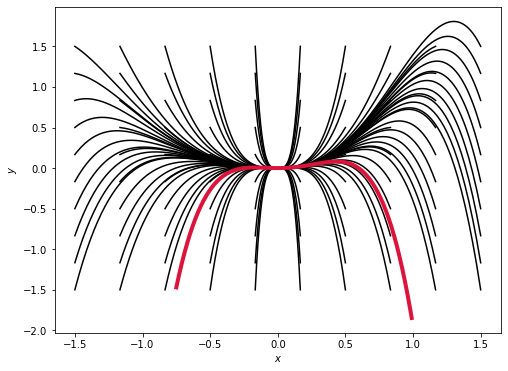
\includegraphics[width=0.5\textwidth]{ssm.png}
    \caption{Solutions to the nonlinear system (\ref{8})-(\ref{9}). Black curves are general solutions from uniformly distributed initial conditions. The red curve is the SSM given by (\ref{ssm}). }
    \label{fig1}
\end{figure}

(e) Obtain an exact reduced-order model for the system.

\emph{Solution}

We obtain the reduced order model by substituting the expression $y=h(x)$, into (\ref{8}). In this case, there is nothing to substitute, the $y$ dynamics does not affect the $x$ dynamics.
$$
\dot{x} = -x.
$$
\end{document}
